\documentclass[polish,polish,a4paper]{report}
\usepackage[T1]{fontenc}
\usepackage[utf8]{inputenc}
\usepackage{babel}
\usepackage{pslatex}
\usepackage{graphicx}
\usepackage{tikz}
\usepackage{pgfplots}
\usepackage{anysize}
\usepackage{pgfgantt}
\usepackage{tabularx}
\usepackage{float}
\usepackage{latexsym,amsmath}
\marginsize{2.5cm}{2.5cm}{0.5cm}{3cm}
\tolerance=6000

\newcommand{\fname}[1]{\sffamily\bfseries\scriptsize #1}

\newcommand{\frontpage}[8]{

\vspace{2cm}

\begin{tabular}{|p{0.72\textwidth}|p{0.28\textwidth}|}
\hline
\multicolumn{2}{|c|}{}\\
\multicolumn{2}{|c|}{{\LARGE #1}}\\
\multicolumn{2}{|c|}{}\\
\hline
\fname{Kierunek} & \fname{Termin}\\
\multicolumn{1}{|c|}{\textit{#2}} & \multicolumn{1}{|c|}{\textit{#3}} \\
\hline
\fname{Imię i nazwisko} & \fname{Prowadzący}\\
\multicolumn{1}{|c|}{\textit{#4}} & \multicolumn{1}{|c|}{\textit{mgr inż. Szymon Datko}} \\
\hline
\end{tabular}

}

\usepackage{listings}
\usepackage{xcolor} % for setting colors

% set the default code style
\lstset{ % General setup for the package
	basicstyle=\small,
	numbers=left,
	frame=tb,
	tabsize=2,
	columns=fixed,
	showstringspaces=false,
	showtabs=false,
	keepspaces,
	commentstyle=\color{red},
	keywordstyle=\color{blue}
}

\title{Sprawozdanie Grafika Komputerowa}
\begin{document}
% #1 - nazwa kursu #2 - kierunek  #3 - termin #4 - temat #5 - problem #6 - data
\frontpage{Grafika komputerowa i komunikacja człowiek-komputer}{Informatyka}{Poniedziałek parzysty 11:00}{Patryk Wlazłyń}
\pagestyle{empty}
\newpage

\pagebreak

\setcounter{chapter}{1}
\chapter*{Podstawy \begin{flushright} 28.10.2019 \end{flushright}}

\setcounter{section}{0}
\section{Opis ćwiczenia}
Ćwiczenie polegało na poznaniu elementarnych operacji dostarczanych dzięki standardowi oraz bibliotece graficznej OpenGL. Jako bibliotekę pomocną do 
tworzenia i zarządzania oknami użyliśmy również biblioteki GLUT (GL Utility Toolkit). Podczas tego ćwiczenia poznaliśmy jak zainicjalizować bibliotekę,
jakie są różnice między używaniem jej na platformie Windows oraz Linux oraz jak generować obraz za pomocą wbudowanych prymitywów w przestrzeni 2D.
Naszym głównym zadaniem do wykonania było narysoowanie dywanu Sierpińskiego, zarówno za pomocą algorytmu rekurencyjnego oraz iteracyjnego. Dodatkowo
miał być on zbudowany z bardzo małych, różnokolorowych kwadratów z drobnymi zniekształceniami.

\section{Rozwiązanie rekurencyjne}
Dywan Sierpińskiego składa się z jednego kwadratu w którym wycinane są dziury w postaci mniejszych kwadratów których bok jest dokładnie 3 razy mniejszy i
rozstawione symetrycznie po każdej ze stron (lewo, prawo, góra, dół) oraz pomiędzy nimi, w rogach (górny-lewo, górne-prawo, dolne-lewo, dolne-prawo).
Łatwo zauważyć, że struktura ta powstaje w takim razie w bardzo ścisłym porządku. Ważnym spostrzeżeniem jest też, że wycinania dokonujemy na obszarach
wielkości dokładnie tej samej co środkowy (głowny) kwadrat, lecz każdy z wyciętych kwadratów jest zwyczajnie 3 razy mniejszy. To pozwala na implementacje
trywialnego algorytmu rekurencyjnego polegającego na wycięciu głównego kwadratu w środku aktualnego obszaru a następnie wycięcie mniejszych, ale zwyczajnie
mniejszch, przesuniętych wzgledem głownego o jego szerokość. Taką procedurę wystarczy powrótrzyć dla każdego nowo utworzonego (mniejszego) z kwadratów
dodając dodatkowo maksymalny poziom zagłębienia i otrzymujemy procedurę rekurencyjną generującą dywan Sierpińskiego.

\section{Rozwiązanie iteracyjne}
Rozwiązanie iteracyjne, najłatwiej jest rozwiązać poprzez spojrzenie na gotowy, wygenerowany dywan Śierpińskiego i zauważenie, że "dziury" konkretnych
wielkości rozstawione są w równych odstępach od siebie i występują regularnie na całej powierzchni dywanu. Ważną informacją jest to, że wieksze dziury
wydają się "przykrywać" te mniejsze. Łącząc te dwie informacje otrzymujemy dwie procedury do wykonania, aby narysować dywan. Równomierne pokrycie 
największego kwadratu dziurami oraz należy zacząć od dziur najmniejszych, tak aby te później rysowane (większe) nadpisały obraz wygenerowany przez
wcześniejsze (mniejsze).

\section{Dodatki}
Losowanie koloru zostało osiągniete poprzez losowanie trzech składowych koloru za pomocą funkcji rand z biblioteki standardowej języka C.
Do rysowania kwadratów została użyta funkcja rysująca dwa przystające do siebie trójkąty. Drobne zniekształcenia, wspomniane w opisie, zostały wprowadzone
poprzez losowanie ich zaraz przed narysowaniem kwadratu - funkcja rysująca kwadrat wprowadza zniekształcenia. Podobnie zostało rozwiązane rysowanie
kwadratów kolorowych.

\section{Implementacja - kod źródłowy}
\lstinputlisting[caption=Dywan Sierpińskiego,language=C++]
{class1.cc}

\pagebreak
\section{Zrzuty ekranu aplikacji}
\begin{center}
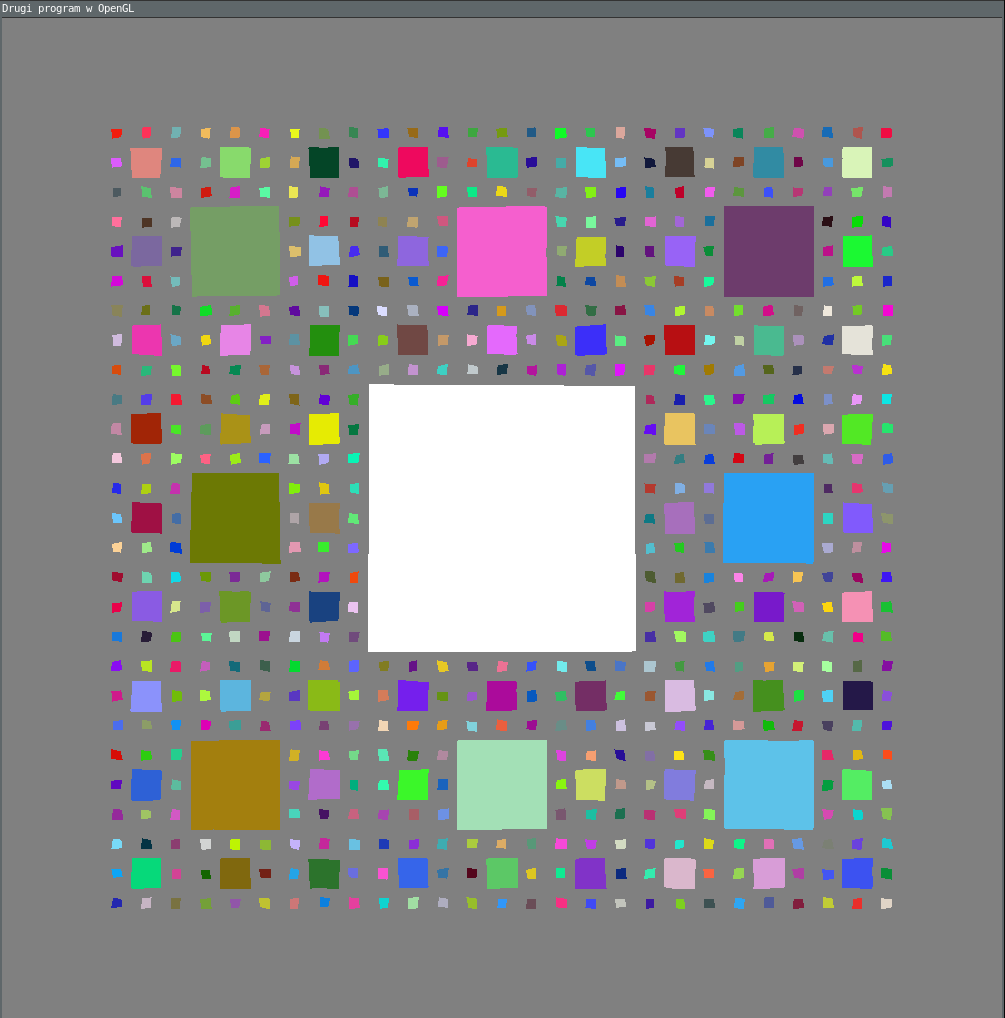
\includegraphics[scale=2]{sierpinski}
\end{center}

\pagebreak
\setcounter{chapter}{2}
\chapter*{Modelowanie obiektów 3-D \begin{flushright} 13.11.2019 \end{flushright}}

\setcounter{section}{0}
\section{Opis ćwiczenia}
Ćwiczenie miało na celu wprowadzenie w zagadnienia związane z modelowaniem i wizualicją scen 3D. Głównymi zagadnieniami przedstawionymi na zajęciach były
transformacje trójwymiarowe na obiektach. Zagadnieniem dodatkowym była obsługa klawiatury do zmiany parametrów animacji. Na ćwiczeniu dane były równanie
otrzymane metodą krzywej Beziera opsujące trójwymiarowy model jajka. Zadaniem autora było narysowanie modelu za pomocą punktów, trójkątów (za pomoca
primitywu GL\_TRIANGLES oraz GL\_TRIANGLE\_STRIP, pokolorowanie oraz włączenie obrotu jajka. Dodatkowo została dodana obsługa klawiatury w celu łatwego
przełączania się pomiędzy trybami wyświetlania.

\section{Rysowanie punktami, oraz siatką}
Po otrzymaniu wzorów które mapują dwu wymiarowe współrzedne na trójwymiarowy punkt rysowanie obiektu jest trywialne.
Podobnie wygląda rysowanie siatki. Wystarczy zmienić tryb rysowania na GL\_LINES.
Poniżej został zamieszczony listing
kodu realizujący to zadanie.

\lstinputlisting[caption=Jajko narysowane punktami,language=C++]
{drawegg_points.cc}

\pagebreak

\begin{figure}[!htb]
\begin{center}
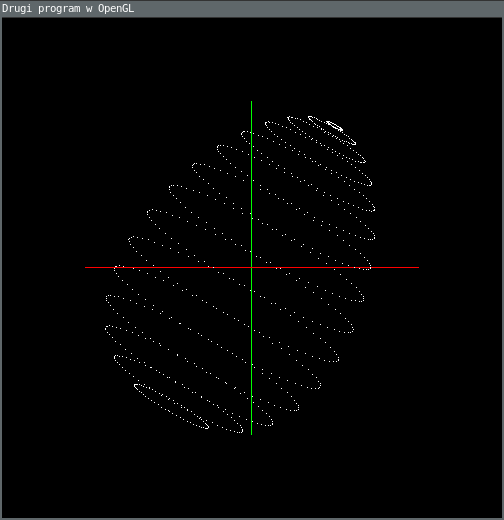
\includegraphics[width=\textwidth]{eggpoints}
\caption{Jajko narysowane za pomocą punktów}
\end{center}
\end{figure}

\pagebreak

\section{Rysowanie trójkątami}
Aby naryswoać jajko za pomocą trójkątów wystarczy ustawić kontekst opengl na rysowanie trójkątami i odpowiednio połączyć sąsiednie punkty, tj.
dla każdego punktu połączyć go z drugim na tym samym poziome, lecz następnego wzdłuż osi X, oraz zamknąc trójkąt łącząc z punktem bedącym nad pierwszym
punktem. Aby jajako składało sie z ładnie przystających trójkątów warto zaraz po tym wykonać juz pierwszy ruch kolejnej iteracji rozpocząć rysowanie
od punktu przesuniętego od początkowego o jeden zarówno w osi X oraz Y. Dzięki obiekt zostanie pokryty idealnie przystającymi trójkątami.
Poniżej został zamieszczony listing kodu realizujący tą funckję.

\lstinputlisting[caption=Jajko narysowane punktami,language=C++]
{drawegg_triangles.cc}

\pagebreak

\begin{figure}[!htb]
\begin{center}
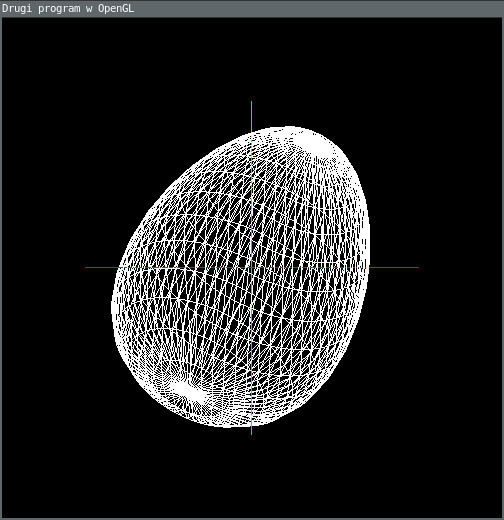
\includegraphics[width=\textwidth]{eggtriangles}
\caption{Jajko narysowane za pomocą trójkątów}
\end{center}
\end{figure}

\pagebreak

\section{Kolorowanie jajka}
Kolorowanie jajka losowymi kolorami odbywa sie poprzed wygenerowanie analogicznej tablicy do tej z zapisanymi punktami, ale tym razem z kolorami dla
każdego koloru, a następnie pobierać ten kolor w czasie rysowania. Inicjalizacja tablicy oraz funckje odpowiedzialne za narysowanie jajka zostały
przedstawione poniżej. Do rysowania użyto prymitywu GL\_TRIANGLES\_STRIP.

\lstinputlisting[caption=Jajko narysowane punktami,language=C++]
{drawegg_tricolo.cc}

\pagebreak

\begin{figure}[!htb]
\begin{center}
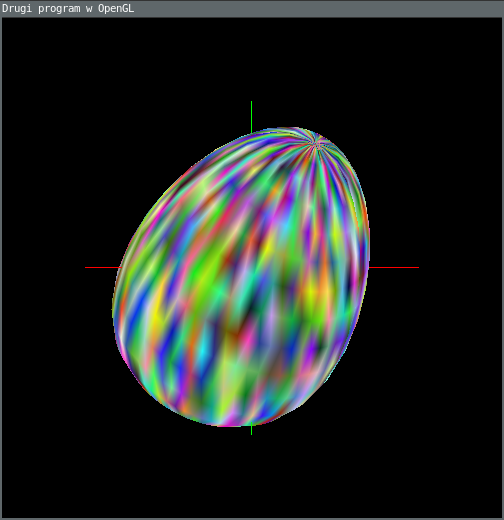
\includegraphics[width=\textwidth]{eggcolor.png}
\caption{Pokolorowane jajko na losowe kolory}
\end{center}
\end{figure}

\pagebreak

\section{Obsługa klawiatury, zmiana parametrów w czasie wykonania}
Aby dodać funckję służącą za obsługę klawiatury należało posłużyć się funkcją z biblioteki GLUT - glutKeyboardFunc(). Jak argument przyjmuje ona wskaźnik
na funkcję, która zostanie wywołana z argumentem jako wciśnięty klawisz (przekonwertowany już na literę ASCII), oraz współrzędne położenia kursora myszy.
Listing opisanych funkcjonalności znajduje się poniżej. Z listingu zostały usuniętę nie istotne fragmenty kodu.

\lstinputlisting[caption=Obsługa klawiatury,language=C++]
{c2_keyboard.cc}

\pagebreak
\setcounter{chapter}{3}
\chapter*{Interakcja z użytkownikiem \begin{flushright} 25.11.2019 \end{flushright}}

\setcounter{section}{0}
\section{Opis ćwiczenia}
Ćwiczenie polegało na przedstawieniu jak realizować interakcję z użytkownikiem przy pomocy sterowania ruchem obiektu i położeniem obserwatora w przestrzeni
3D za pomocą myszy. Dodatkowo przedstawione zostały sposoby prezentacji obiektów trójwymiarowych w rzucie prostokątnym. Na zajęciach został przedstawiony
koncept poruszania kamerą. Da się to osiągnąc za pomocą poruszania wszystkimi obiektami zamiast kamerą, co w efekcie da takie same rezultaty. Poruszanie
obiektami w OpenGL jest relatywnie proste. Wykorzystywane są do tego macierze transfrmacji, ktore ustawia się przed rysowaniem. Dzięki takiemu zabiegowi
wszystko co bedzięmy rysować, najpierw będzie poddane transformacji. Co oznacza, że same procedury rysowania mogą być takie same, a jedynie ustawia się
główną funkcję renderującą w odpowiednim kontekście. Należy jednak pamiętać, że modyfikacje macierzy transformacji nie nadpisują dotychczasowych wartości,
a wykonują mnożenie aktualnej macierzy transformacji przez przekazaną macierz. Co oznacza, że ustawiana transformacja zostanie dołożona do istniejącej.
Aby zaaplikować tylko jedną z transormacji, należy najpierw wyczyścić stan macierzy transformacji za pomocą glLoadIdentity(), która wczyta macierz
jednostkową a dopiero później wpisać kolejną. Wszystkie operacje wykonywane były na modelu imbryczka, narysowanego przez funkcję glutWireTeapot();

\section{Transformacje}
Do kontrolowania zachowania położeniem kamery posłużyły funckje: gluLookAt, glRotatef, glScalef, oraz glTranslatef.
Które kolejno służą do ustawienia punktu na który skierowana jest kamera, zaaplikowanie transformacji obrotu, zaaplikowanie transformacji skalowania
oraz zaaplikowania transformacji przesunięcie. Prawie wszystkie parametry wspomnianych funkcji dodatkowo były wywoływane z argumentami, które
można było modyfikować w trakcie działania programu za pomocą klawiatury w dokładnie ten sam sposób co w poprzednich zadanich.
Warto jeszcze zauważyć, że kolejność transformacji ma znaczenie, gdyż odpowiada ono mnożeniu przez odpowiednie macierze.
Wszystkie transformację nakładane są w funkcji RenderScene w sposób w jaki zostało to pokazane na poniższym listingu.
Zmienna viewer to tablica która przechowuje informację na temat położenia kamery. Używana jest jako argument do funkcji gluLookAt.
Jej pozycja wyliczana jest na podstawie wzoru, który jako argumenty przyjmuje elewację oraz azymut.
Oba te parametry podlegają modifykacji przy pomocy klawiatury i myszy, co pozwala na poruszanie kamerą.

\pagebreak
\lstinputlisting[caption=RenderScene z wykorzystaniem transformacji (symulacja ruchu kamery),language=C++]
{c3_renderscene.cc}

\pagebreak

\section{Przeciwdziałanie dowracania się obiektu przy dużym kącie obrotu}
Pozostaje jednak jeden problem do rozwiązania. Gdy obrót kamery ustawimy na zbyt duży kąt tj, od 180 do 270 (mod 360) to renderowany model zaczyna być
rysowany odwrotnie ("do góry nogami", jeżeli ma to sens dla imbryczka). Powodem tego jest zmiana znaku wektora wskazującego od kamery do obserwowanego
punktu. Aby temu zapobiec, należy w wspomnianym zakresie, ręcznie zmienic znak poprzed podanie jako argumentu do gluLookAt wartości -1.0 jako 8.
argumentu. Tak zmodyfikowana funkcja już poprawnie wyświetla modele niezależnie od wartości kątu elewacji i azymutu.

\lstinputlisting[caption=Kontrolowanie parametrów obrotu za pomocą myszy,language=C++]
{c3_keyboard.cc}

\pagebreak

\section{Zrzuty ekranu aplikacji}
\begin{center}
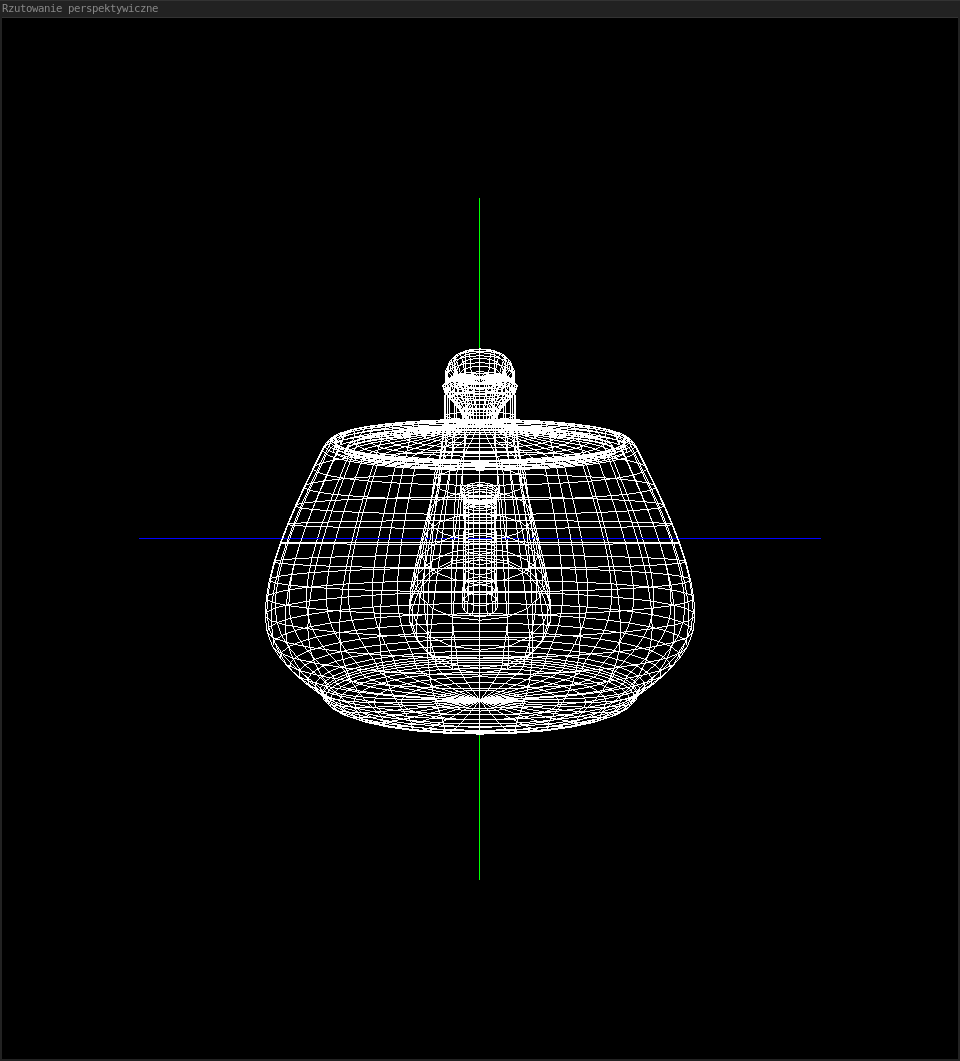
\includegraphics[width=\textwidth=2]{imbryk1}
\end{center}

\begin{center}
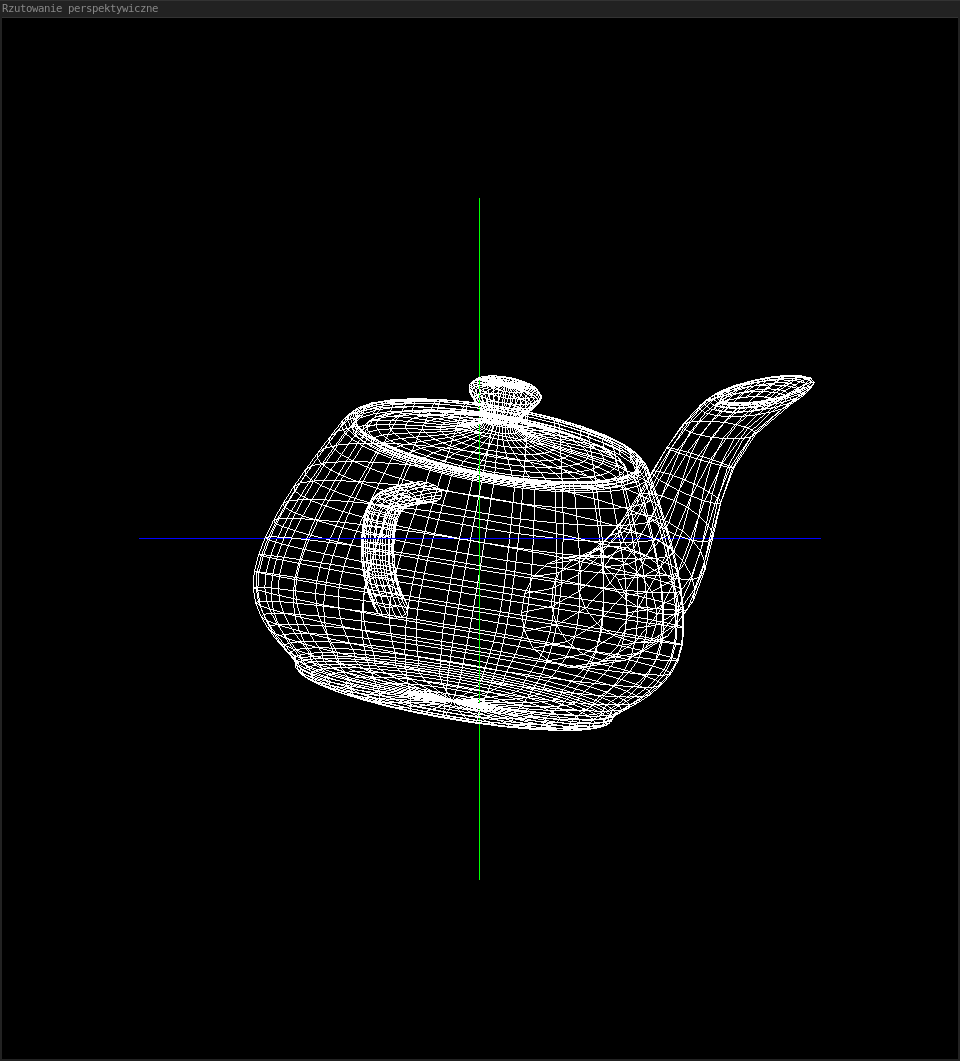
\includegraphics[width=\textwidth=2]{imbryk2}
\end{center}

\begin{center}
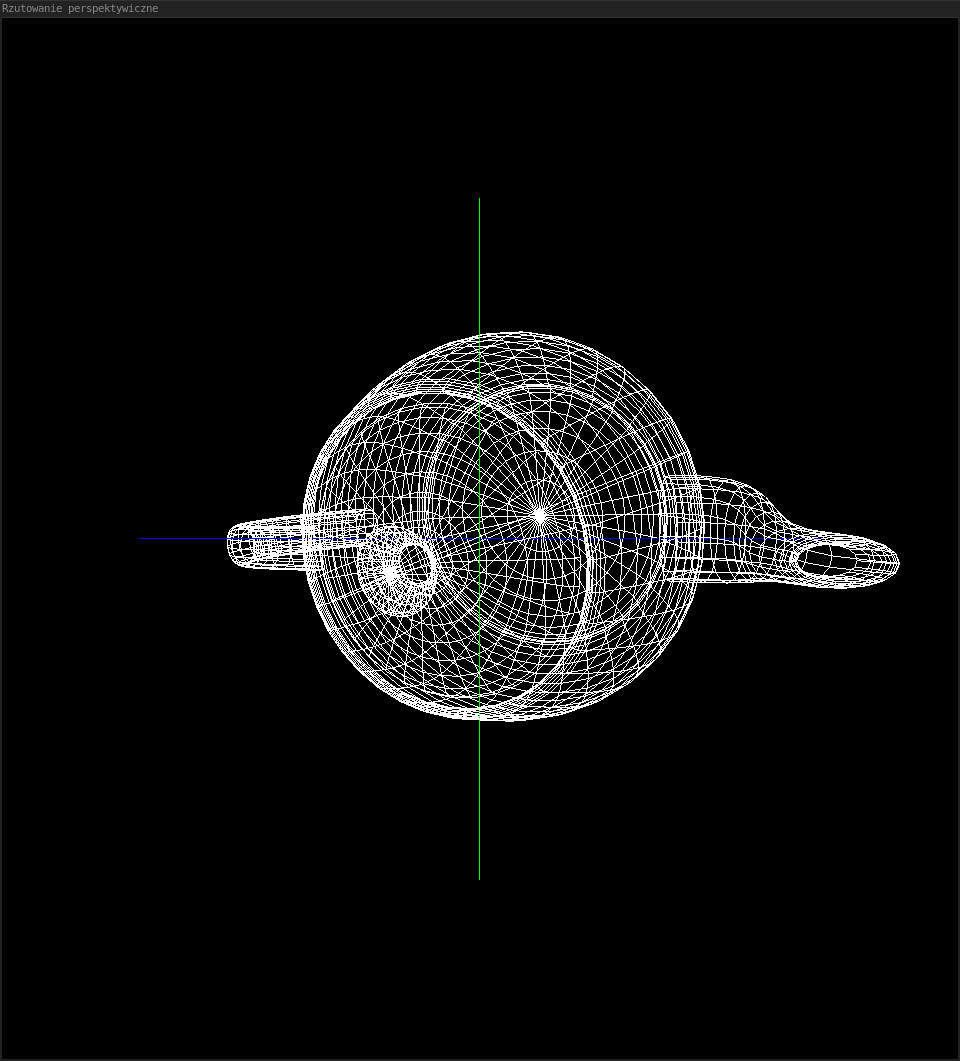
\includegraphics[width=\textwidth=2]{imbryk3}
\end{center}

\begin{center}
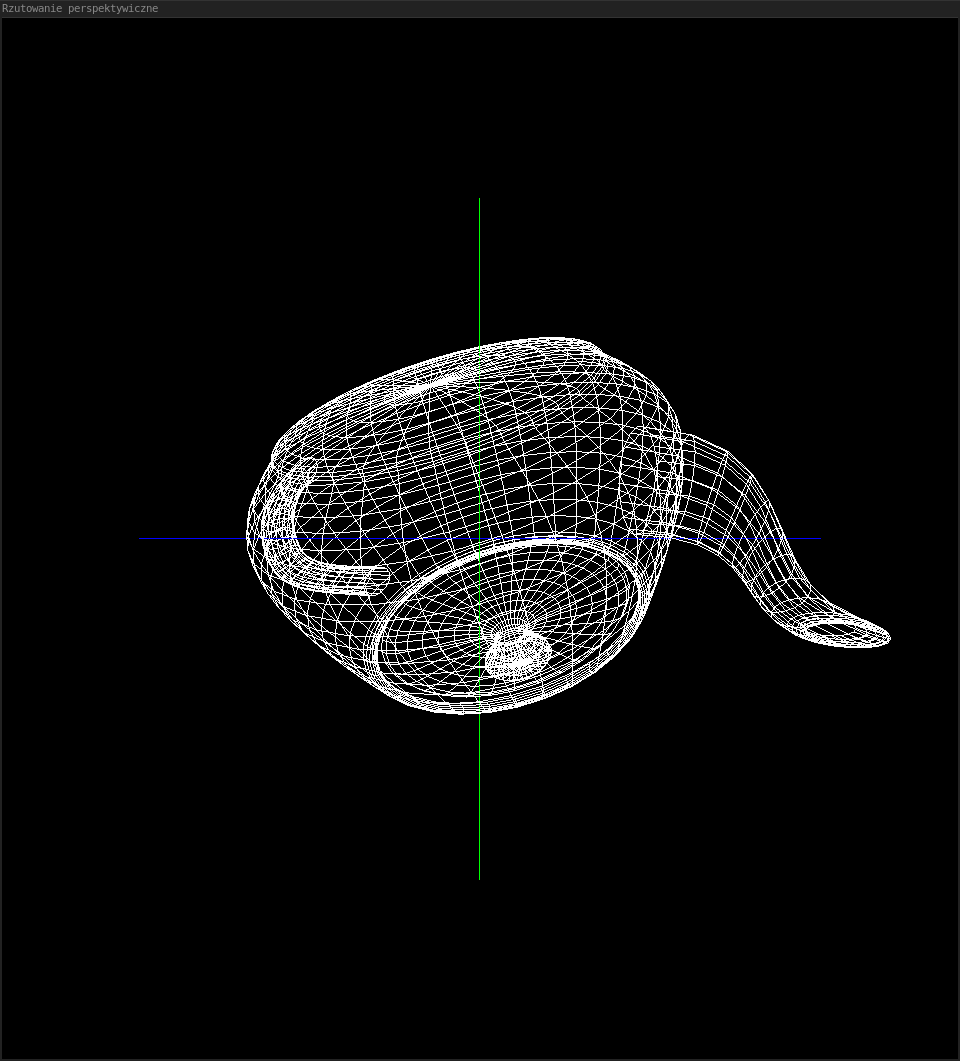
\includegraphics[width=\textwidth=2]{imbryk4}
\end{center}

\pagebreak

\setcounter{chapter}{4}
\chapter*{Oświetlanie scen 3-D\begin{flushright} 09.12.2019 \end{flushright}}

\setcounter{section}{0}
\section{Opis ćwiczenia}
\par Na tym ćwiczeniu zostały przedstawiene możliwości generowania oświetlenia za pomocą biblioteki OpenGL.
Wprowadzone zostały funkcje włączania oświetlenia, a także te od nadawania im różnych cech.
Oświetlenie w rzeczywistości jest bardzo skomplikowanym zjawiskiem i jego pełne symulowanie jest zbyt drogie.
W tym celu w standardzie OpenGL zdefiniowano trzy cechy jakie symuluje się wprowadzając na scene oświetlenie, które dają relatywnie dobry efekt
i co najważniejsze - są łatwo osiągalne na współcześnie dostępnym sprzęcie.
Światło w OpenGL składa się z trzech komponentów - ambient, diffuse i specular, które razem dają model Phonga.
Komponent ambient opisuje zjawisko polegające na tym, że obiekty w sąsiedztwie dowolnego oświetlenia nigdy nie są kompletnie czarne.
Ten komponent zatem nadaje odpowiednio przyciemniony kolor danemu obiektowi.
Komponent diffuse nadaje oświetlenia obiektowi zależnie od tego jak dana jego część jest dla tego źródła "widoczna".
Nadaje to efekt cieniów w miejscach mniej bezpośrednio nachylonych w kierunku światła.
Ostatni komponent to sepcular, który wytwarza efekt połysku w miejsach najbardziej skierowanych w strone źródła światła.
Aby wytworzyć ostateczny efekt, wszystkie te komponenty łączone są w jedno.
Komponent diffuse oraz specular aby ocenić jak bardzo dany obiekty (a raczej jego fragment) jest nachylony w stronę źródła światła wykorzystują
wektory normalne tych powierzchni.
Zadaniem do zrealizowania podczas zajęć było dodanie drugiego źródła światła do sceny, dodanie możliwości poruszania światłem, dodanie możliwości
zmiany składowych światła, dodanie wspomnianych wektorów normalnych do modelu jajka, oraz, jak się następnie okazało - "naprawa" wektorów normalnych
dla punktów znajdujących się z tylnej strony jajka (bez tego, tylko połowa jajka była widoczna).

\pagebreak
\section{Dodanie drugiego źródła światła}
Dodanie światła do sceny jest trywialne. Wystarczyło powielić komponenty ambient, diffuse i specular, oraz zainicjalizować światło nowymi wartościami.
Listing kodu realizujący tą funckjonalność został zamieszczony poniżej.

\lstinputlisting[caption=Dodanie dwóch źródeł swiatła,language=C++]
{c4_secondlight.cc}

\pagebreak
\section{Dodanie możliwości poruszania światłem}
Możliwość poruszania świtałem została dodana podobnie do poprzednich zadań. Do funkcji obsługującej wejście klawiatury zostały dołożone odpowiednie
fragmenty manipulujące komponentami oraz położeniem światła. Listing opisywanego kodu znajduje się poniżej.

\lstinputlisting[caption=Kontrolowanie położenia źródeł swiatła za pomocą klawiatury,language=C++]
{c4_movelight.cc}

\pagebreak
\section{Naprawa wektorów normalnych z tyłu jajka}
Problemem powstałym przy wyliczaniu wektorów normalnych z podanego na zajęciach wzoru, było to, że wektory normalne dla fragmentów z tyłu jajka nadal
wskazywały ten sam kierunke co wektory normalne, przednie.
Rozwiązaniem tego problemu było (dla punktów odpowiednio od połowy jajka) zmiana znaku
otrzymanych wektorów na przeciwne. Listing zawierający kod znajduje się poniżej.

\lstinputlisting[caption=Kontrolowanie położenia źródeł swiatła za pomocą klawiatury,language=C++]
{c4_norms.cc}

\pagebreak
\section{Zrzuty ekranu aplikacji}
\begin{center}
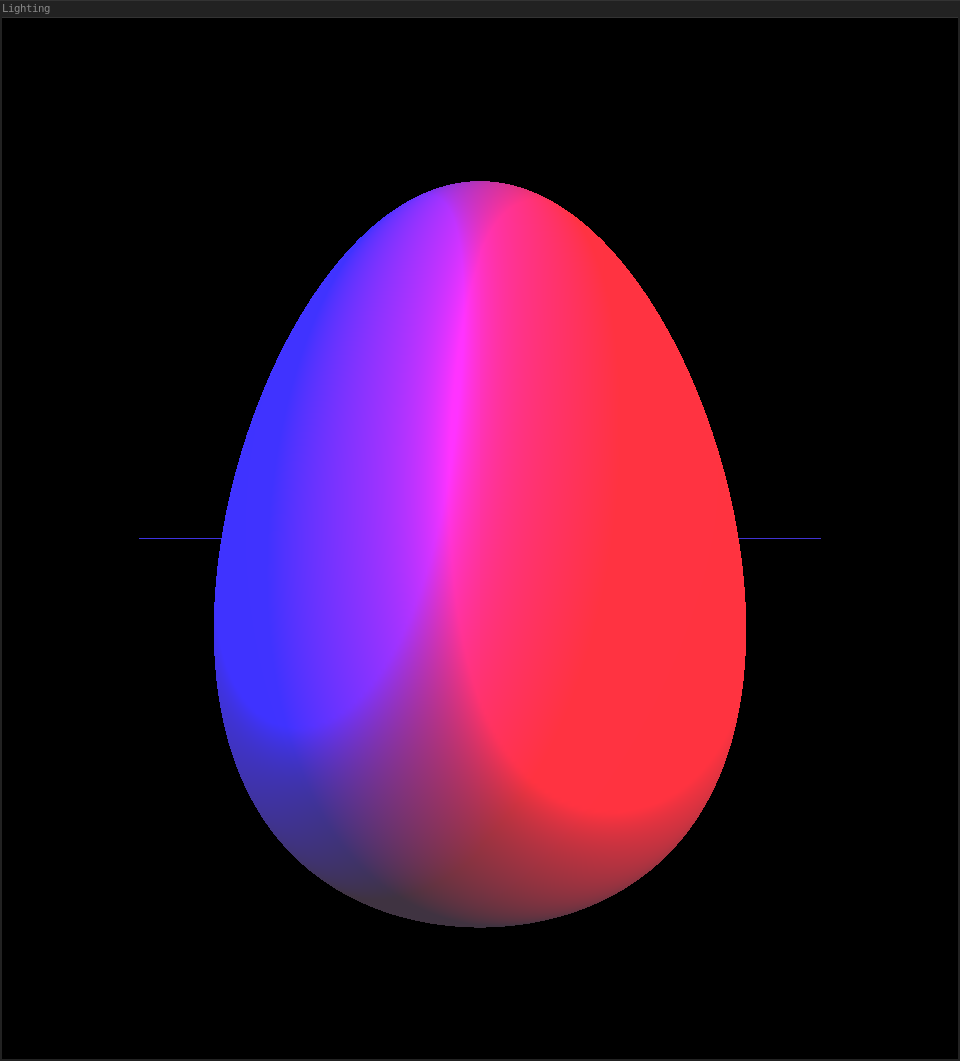
\includegraphics[scale=2]{egg_light1}
\end{center}

\pagebreak
\begin{center}
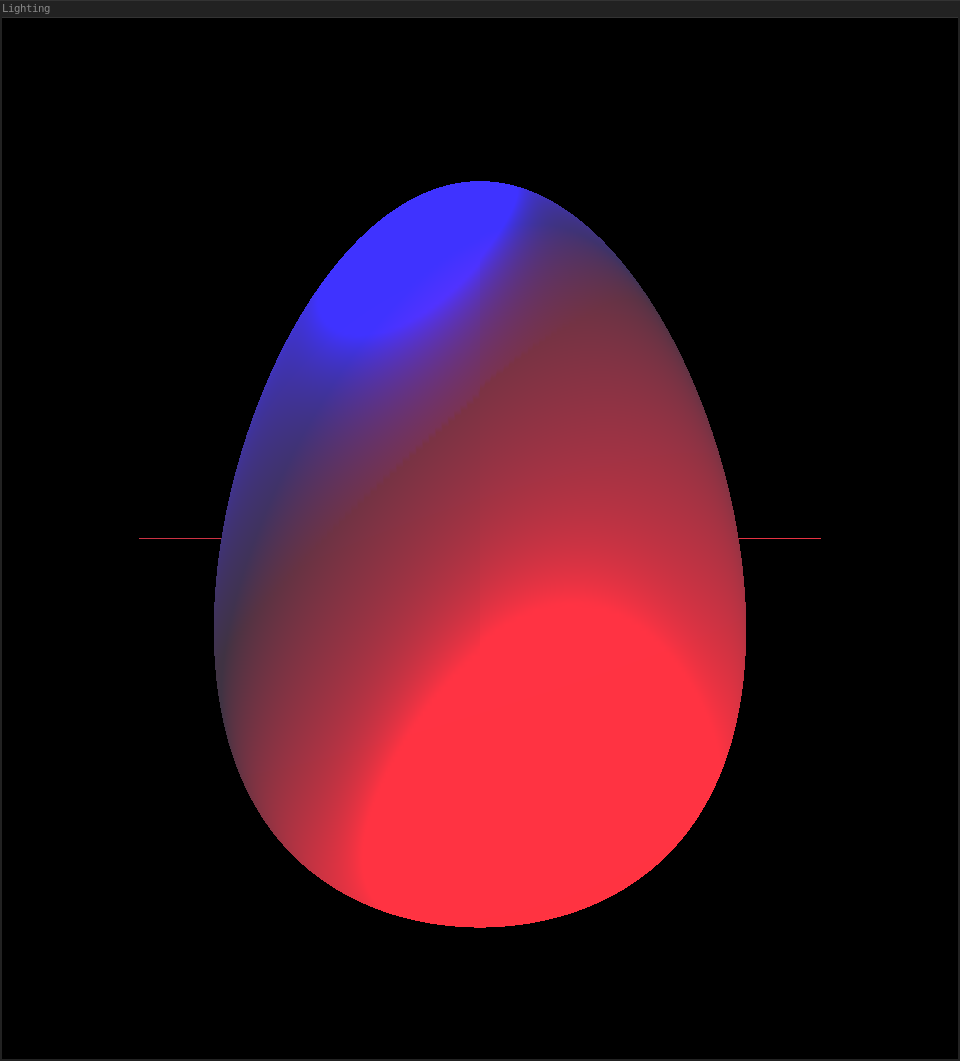
\includegraphics[scale=2]{egg_light2}
\end{center}

\pagebreak
\begin{center}
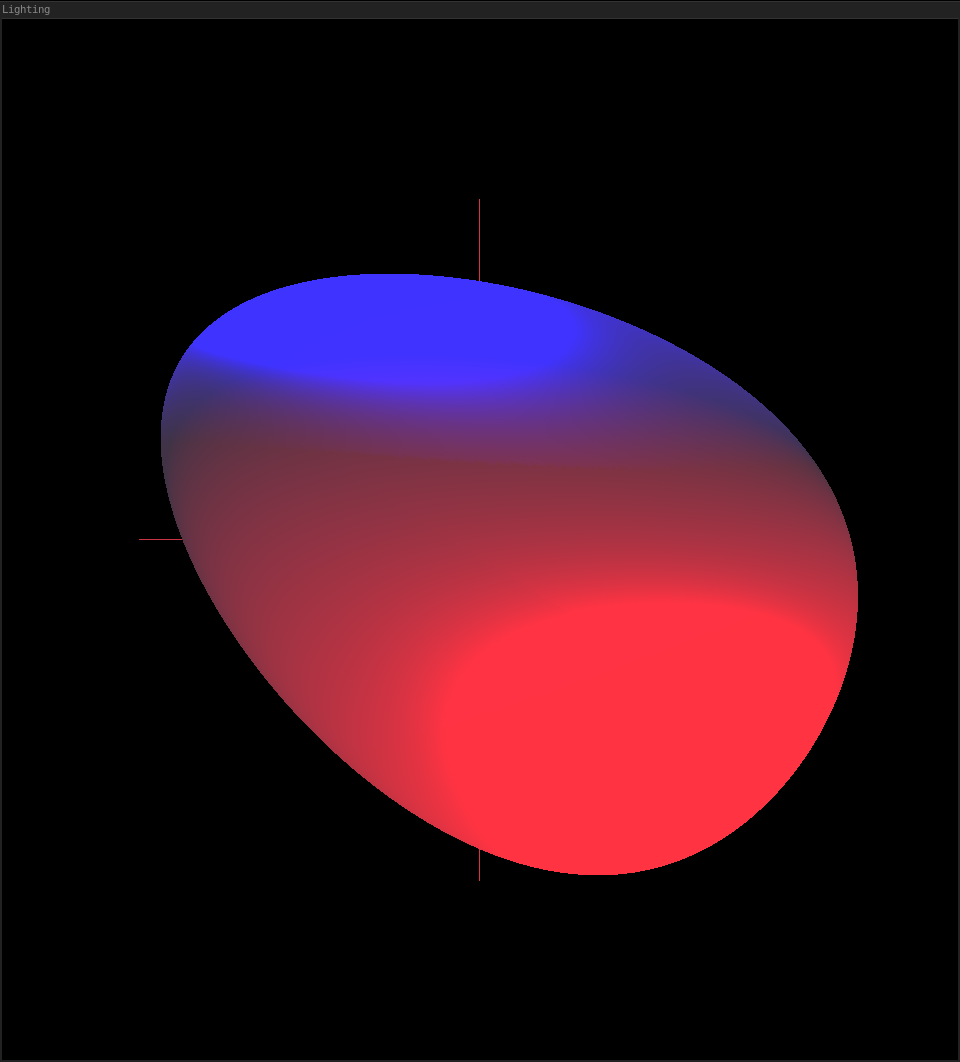
\includegraphics[scale=2]{egg_light3}
\end{center}

\pagebreak

\setcounter{chapter}{5}
\chapter*{Teksturowanie powierzchni obiektów\begin{flushright} 09.12.2019 \end{flushright}}

\setcounter{section}{0}
\section{Opis ćwiczenia}
Celem ćwiczenia było przedstawienie możliwości teksturowania powierzchni obiektów w bibliotece OpenGL.
Teksture nakładamy na narysowany trójkąt wybierając trzy punkty na tekstrurze, która zostanie rozciąganieta w taki sposób aby pokryć rysowany trójkąt.
Po wczytaniu do obrazu w pamieci odwołujemy sie używając współrzędnych znormalizowanych (tj. od 0.0 do 1.0), w obu wymiarach.
Pierszym z zdań było użycie kodu z poprzednich zadań w celu obrotu rysownego obiektu za pomocą myszy.
Pierwszym obiektem do narysowania i oteksturowania był płaski trójkąt.
Drugim obiektem był ostrosłup, którego można narysować za pomocą 6 trójkątow ( 2 w podstawie i 4 na scianach bocznych ).
Ostatnim obiektem do narysowania i pokrycia teksturą był model jajka z poprzednich zajęć.
Gotowe tekstury przygotowane były już przez prowadzącego, ale również jako jeden z punktów ćwiczenia było przygotowanie własnej tekstury.
Wybór padł na obrazek z wizerunkiem fikcyjnej postaci Yui Hirasawa z jednej z Chińskich bajeczek, ze względu na wzbudzanie przez nią skrajnych emocji
u ludzi ją widzących, oraz, że akurat przypadkiem autor miał już gotową kopię na dysku.

\section{Trójkąt i ostrosłup}
Rysowanie trójkąta jest trywialnie proste. Wystarczy użyć gotowej funkcji z biblioteki OpenGL do rysowania w trójwymiarze.
Nałożenie na niego tekstury polega na wybraniu wierzchołka na dwuwymiarowej teksturze zaraz przed rysowaniem każdego wierzchołka trójkąta.
W ten sposób tekstura zostanie odpowiednio pobrana z zaznaczonego obszaru oraz rozciągnięta na rysowanym trójkącie, tak aby pokryć go całego.
Rysowanie ostrosłupa nie jest niczym bardziej skomplikowanym. Jedynie należy powielić opisane operacje, tak aby rysowane trójkąty stworzyły ostrosłup.
Listing kody realizującego tą funkcjonalność znajduje się poniżej.

\lstinputlisting[caption=Rysowanie obiektu oteksturownego trójkąta oraz ostrosłupa,language=C++]
{c5_tri.cc}

\begin{center}
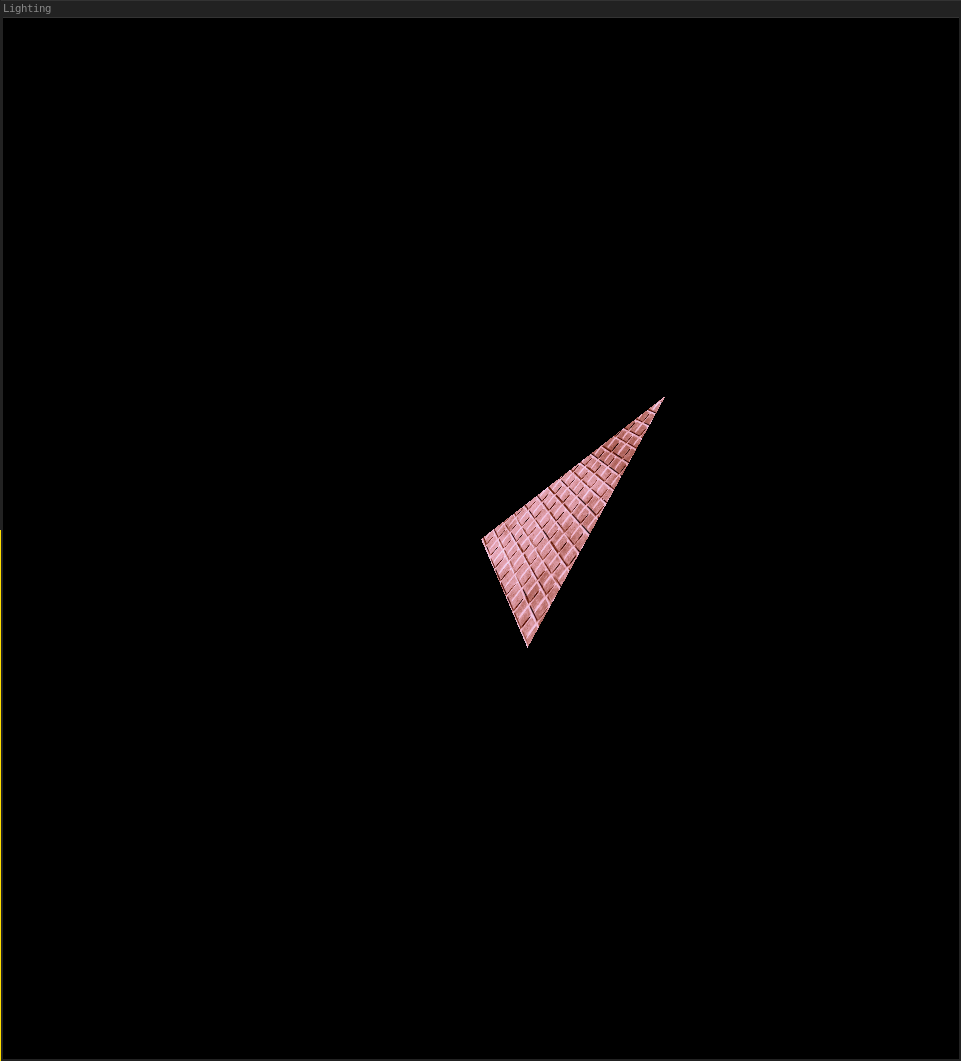
\includegraphics[scale=1.5]{textri}
\end{center}

\begin{center}
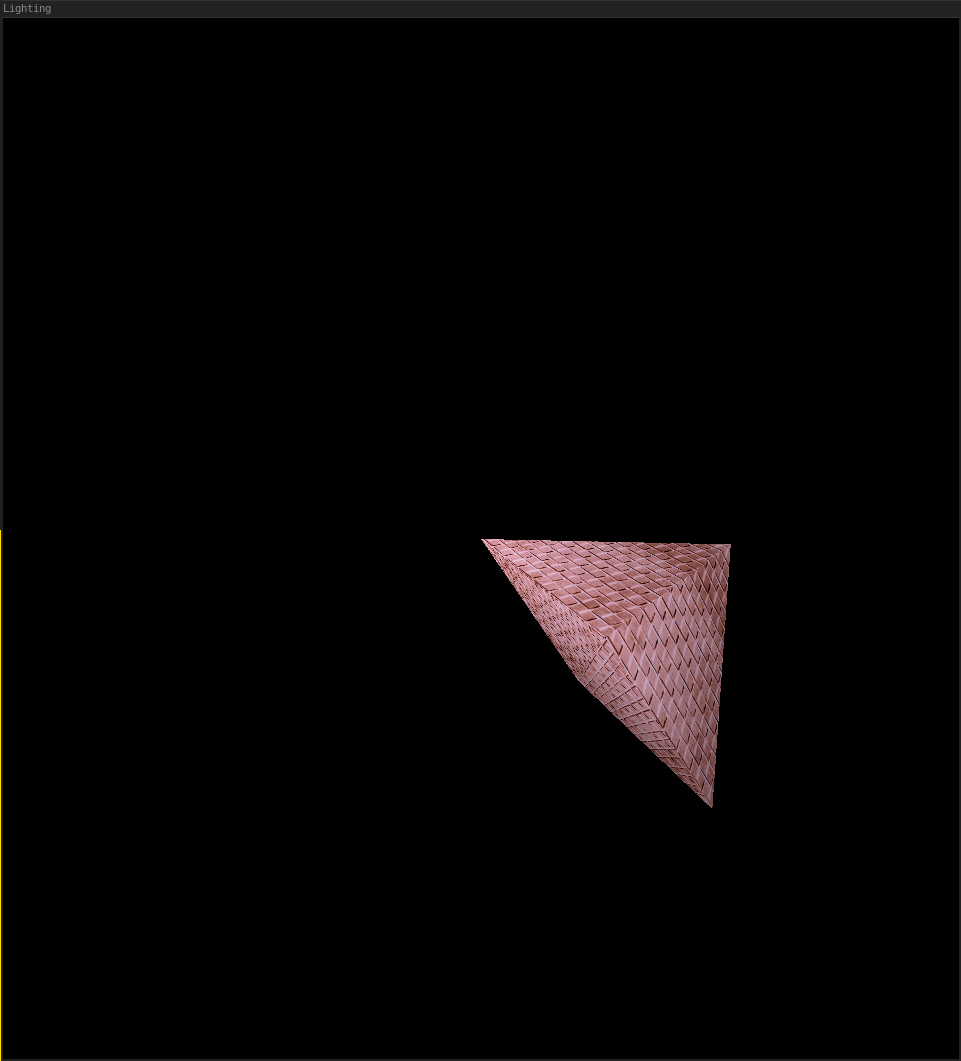
\includegraphics[scale=2]{texpyra}
\end{center}

\begin{center}
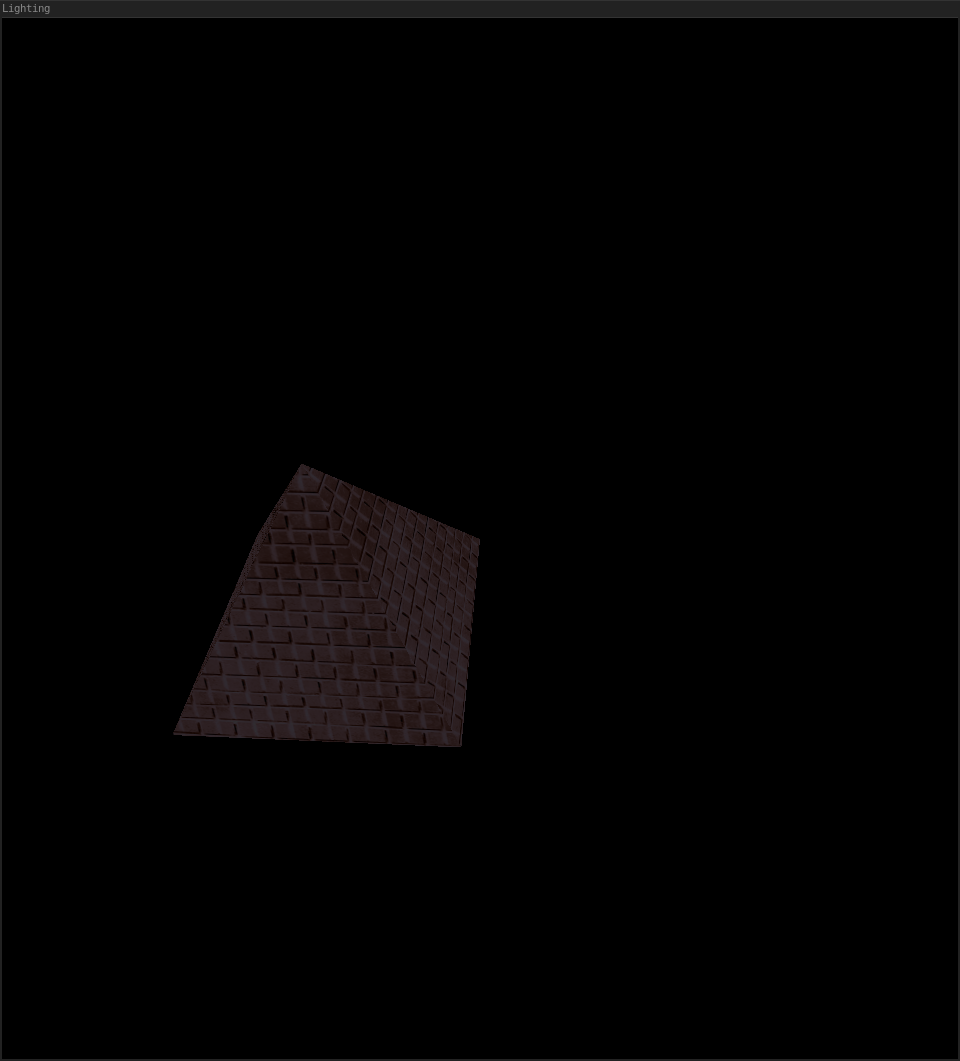
\includegraphics[scale=2]{texpyra2}
\end{center}

\begin{center}
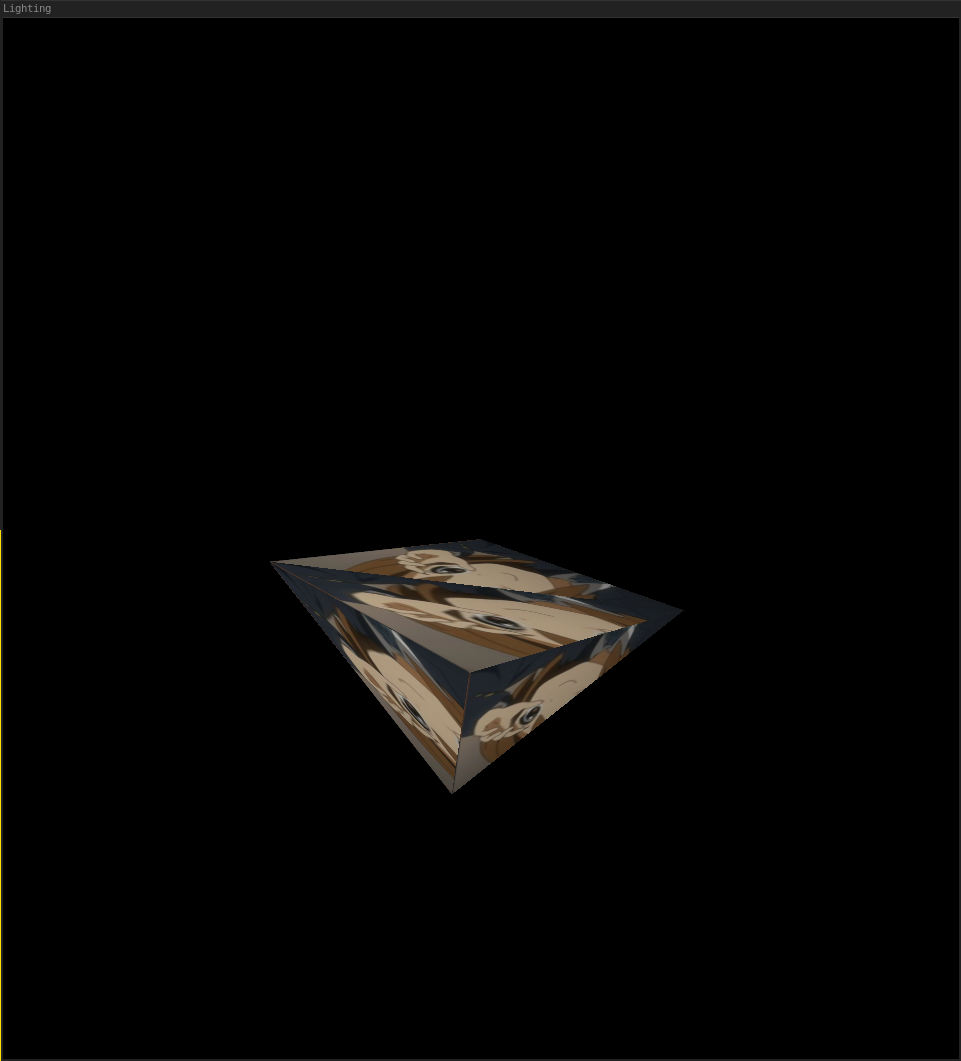
\includegraphics[scale=2]{yuipyra.png}
\end{center}

\pagebreak
\section{Jajko}
Do rysowania jajka z trójkątów został użyty kod z poprzednich zajęć.
W trakcie realizowania tej częsci zadania autor napotkał kilka trudności.
Po pierwsze - jajko narysowane za pomocą samodzielnie przygotowanej tekstury wyglądało nieestetycnie.
Przez to w jaki sposób rysowane jest jajko istnieje zauważalna różnica w odległościach miedzy punktami modelu poziomie oraz w pionie.
Powodowało to, że tekstura była bardzo spłaszczona, a słodziutki wizerunek Yui, słabo widzoczny.
Aby rozwiązać ten problem autor postanowił rysować w poziomie co drugi punkt, z szerszymi trójkątami.
Ta prosta operacja dała bardzo dobre rezultaty.
Kolejnym problemem okazało się to, że jajko z jednej ze stron wogóle się nie rysuje.
Jak sie po chwili okazało była to wina face cullingu w OpenGL i tego, że tylnia powierzchnia jajka rysowana była tyłem do obserwatora, przez co nie była
rysowana na ekranie. Aby sobie z tym poradzić wystarczyło połowe jajka rysować w stronę pierwotnego położenia obserwatora, a drugą skierowaną w kierunku
przeciwnym. Ostatnim problemem okazała się być odwrócona o 180 stopni tekstura z jednej strony jajka.
Powodem takiego zachownia był sam sposób w jaki rysowane jest jajko.
Autor postanowił poradzić sobie z tym problemem rozszerzając własną teksturę o odbicie w poziomie i korzystanie z drugiej połówki tekstury w trakcie
rysowania. Listing kodu odpowiedzialny za opsiywaną funkcjonalność znajduje się poniżej.

\lstinputlisting[caption=Rysowanie obiektu oteksturownego trójkąta oraz ostrosłupa,language=C++]
{c5_texegg.cc}

Powielenie tekstury w celu łatwej zmiany orientacji (oczywiście autor nie miał na myśli zmiany orientacji seksulanej poprzez powielenie obrazków z 
wizerunkiem Yui).

\begin{center}
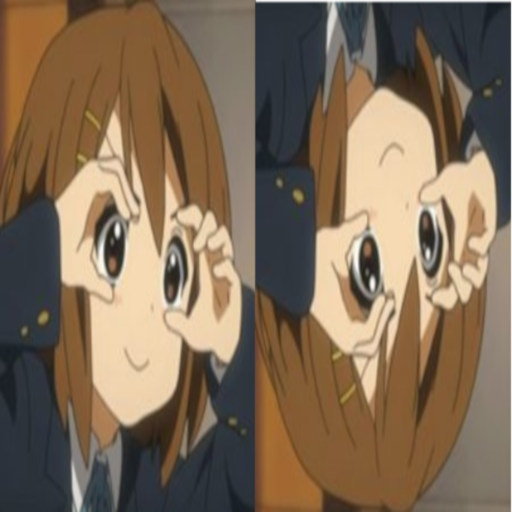
\includegraphics[scale=2]{yui}
\end{center}

\pagebreak
\section{Zrzuty ekranu aplikacji}

\begin{center}
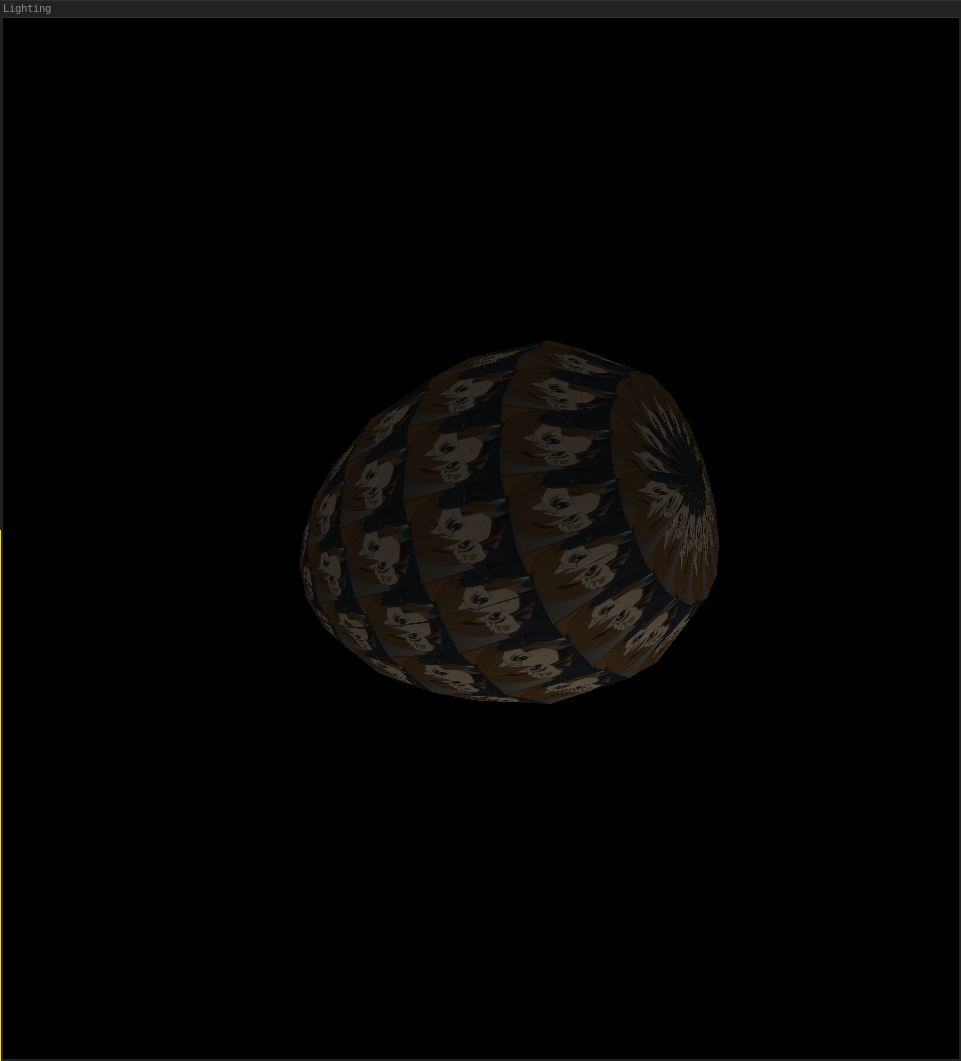
\includegraphics[scale=2]{yuiegg1.png}
\end{center}

\begin{center}
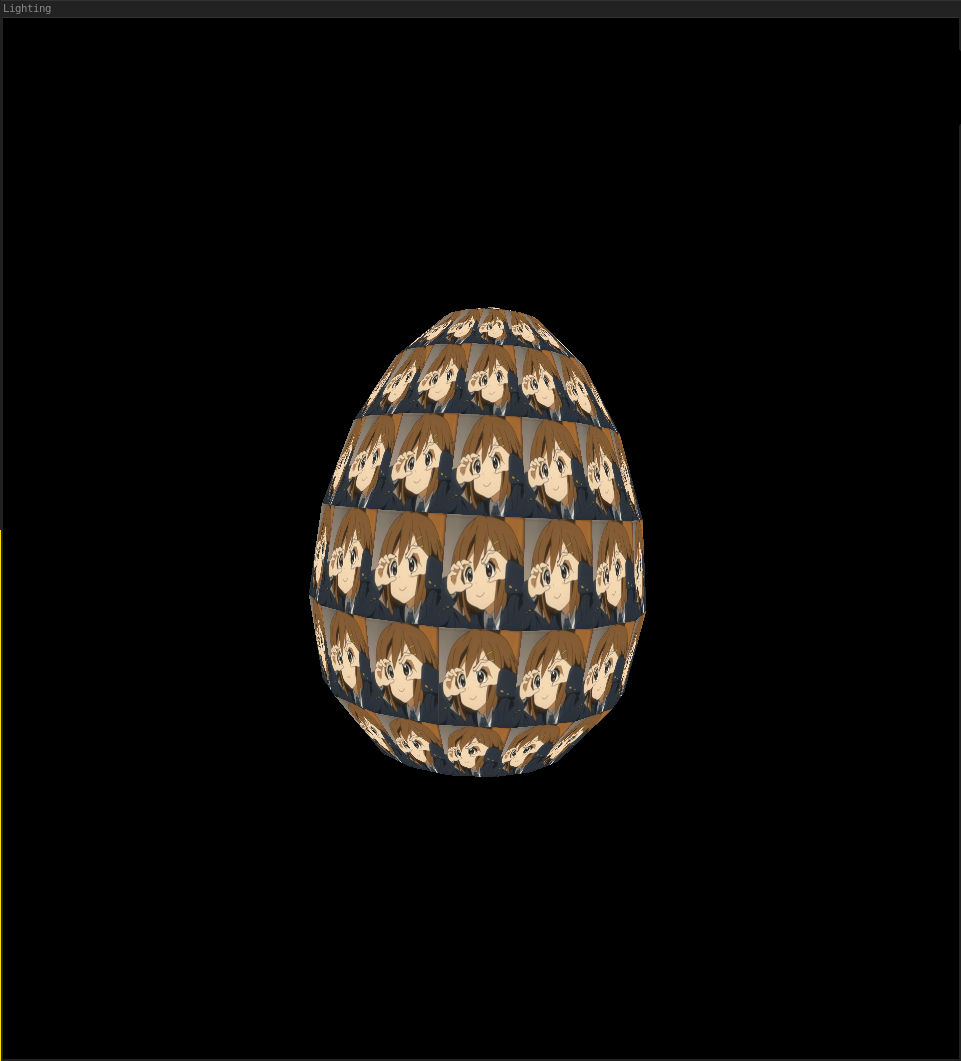
\includegraphics[scale=2]{yuiegg2.png}
\end{center}

\begin{center}
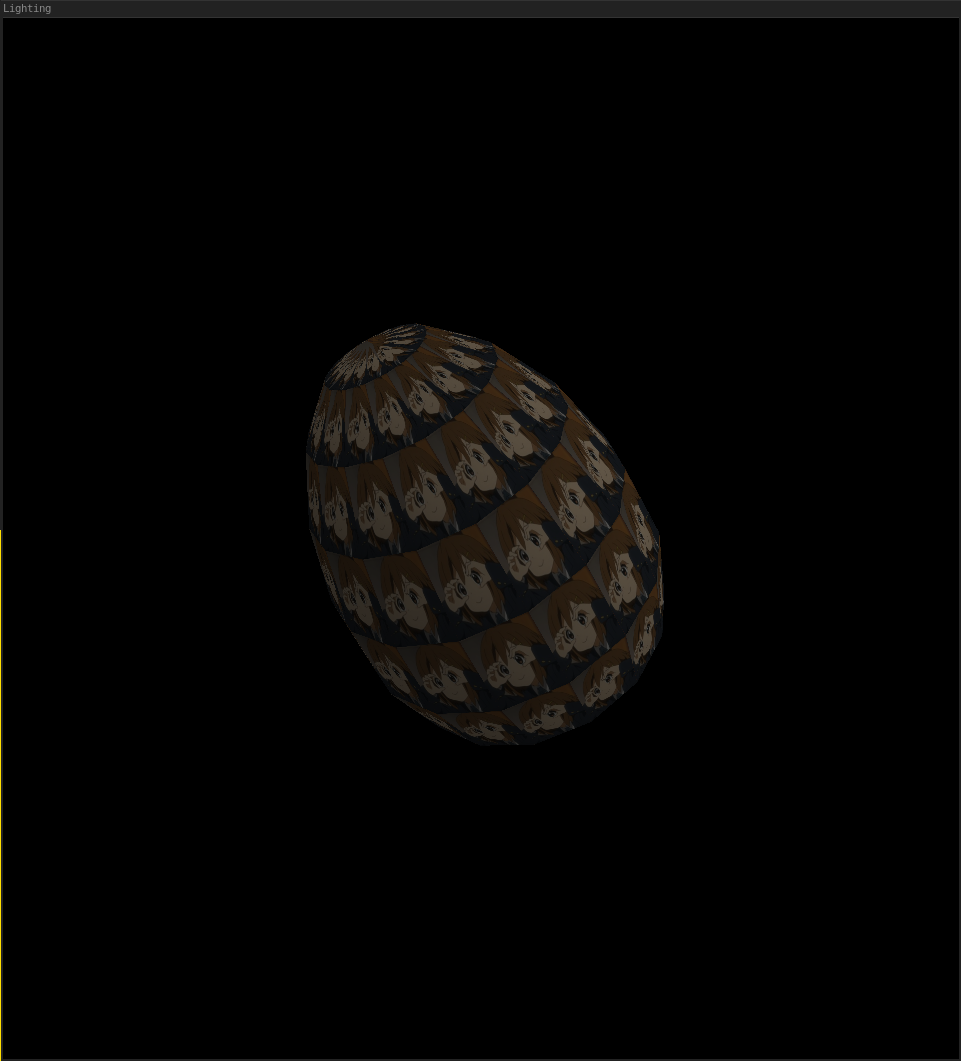
\includegraphics[scale=2]{yuiegg3.png}
\end{center}

\end{document}

